\newcommand\red[1]{
  \node [circle,fill=red,text=black] {\textbf #1}
}

\newcommand\blue[1]{
  \node [circle,fill=blue,text=white] {\textbf #1};
}

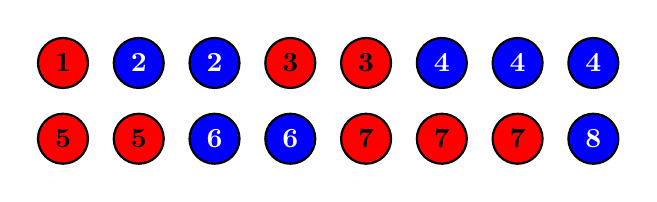
\begin{tikzpicture}

\matrix (m) [nodes={draw, thick}, row sep=0.3cm, column sep=0.3cm] {
  \red{1}; &
  \blue{2}; &
  \blue{2}; &
  \red{3}; &
  \red{3}; &
  \blue{4}; &
  \blue{4}; &
  \blue{4}; \\
  \red{5}; &
  \red{5}; &
  \blue{6}; &
  \blue{6}; &
  \red{7}; &
  \red{7}; &
  \red{7}; &
  \blue{8}; \\
};

\end{tikzpicture}
